\documentclass[11pt,a4paper]{article}
\usepackage[T1]{fontenc}
\usepackage[margin=2.3cm]{geometry}
\usepackage{amsmath,amssymb}
\usepackage{graphicx}
\usepackage[dvipsnames]{xcolor}
\usepackage{enumitem}
\usepackage[colorlinks=true,linkcolor=blue,urlcolor=blue]{hyperref}
\setlength{\parskip}{0.6em}
\setlength{\parindent}{0pt}
\begin{document}

\begin{center}{\LARGE\bfseries openascent}\\[0.4em]{\large Fly a rocket launch trajectory to orbit with staging, in three sessions.}\\[0.2em]\small PAN IIT OSS explainer \textbullet{} higher secondary to advanced undergraduate (levels 4-6)\end{center}

\section*{Why this exists}
A rocket must climb and turn to reach orbit, and staging drops dead weight on the way. This explainer follows the idea from the rocket equation and staging, through the gravity and drag losses of a vertical climb, to a two-stage gravity-turn ascent into a 200 km orbit, using only Newton's laws, momentum conservation and inverse-square gravity.

\section*{The end goal}
Fly a rocket launch trajectory to orbit with staging: know how much delta-v orbit needs, where the losses come from, why the rocket turns over and why it drops stages, and check a simulation against the laws it must obey. The same ideas apply to sounding rockets, missiles, landers and every launch vehicle.

\section*{How the three sessions build up}
\begin{enumerate}[nosep]
\item \textbf{Session 1: The rocket equation and staging} (Level 1, conceptual interactive model, 60 min).
\item \textbf{Session 2: Straight up: gravity and drag losses} (Level 2, mathematical engineering model, 75 min).
\item \textbf{Session 3: Fly to orbit with a gravity turn and staging} (Level 3, simulation and validation, 90 min).
\end{enumerate}

\section{Session 1: The rocket equation and staging}

\subsection*{A. Real-world problem}
A launch vehicle like India's PSLV has a lift-off mass of roughly 300 tonnes, yet it places only one or two tonnes into a low orbit. Almost everything else is propellant thrown out of the nozzles during the climb, plus tanks and engines that are thrown away in the sea. Why does a rocket need so much propellant to reach orbit, and why is it built in stages that are dropped on the way up? (General education only: this is a simplified model, not a launch vehicle design method.)

\subsection*{B. Concept and theory}
A rocket moves by throwing mass backwards. When a small mass dm leaves at exhaust speed ve relative to the rocket, momentum conservation says the remaining mass m speeds up by dv = ve dm / m. Adding up these small pieces from the full (lift-off) mass m0 to the empty (burnout) mass mf gives the Tsiolkovsky rocket equation, delta-v = ve ln(m0 / mf). Engines are rated by their specific impulse Isp in seconds; the exhaust speed is ve = Isp x g0 with g0 = 9.80665 m/s2. The logarithm is harsh: each extra ve of speed needs the mass ratio multiplied by e = 2.718 again. A low circular orbit needs a sideways speed v = sqrt(G M / r), about 7.8 km/s at 200 km; gravity and air on the way up add roughly 1.5 to 2 km/s, so a typical budget is about 9.4 km/s. Staging helps because once a stage's propellant is gone, its empty tanks and engines (the dry mass) are dead weight. A two-stage rocket burns stage 1, drops it, and then stage 2 only has to push itself and the payload, so each stage has a good mass ratio and the delta-v values add.

\begin{itemize}[nosep]
\item ve: effective exhaust speed, Isp x g0 (m/s)
\item g0: standard gravity, 9.80665 (m/s2)
\item m0, mf: mass at the start and at the end of a burn (kg)
\item delta-v: ideal speed change of a burn (no gravity, no air) (m/s)
\item G M (mu): Earth's gravitational parameter, 3.986 x 10\textasciicircum{}14 (m3/s2)
\item r, h: distance from Earth's centre, and altitude r - 6371 km (m)
\end{itemize}

\begin{equation*}
v_e = I_{sp}\, g_0
\end{equation*}

\begin{equation*}
\Delta v = v_e \ln\frac{m_0}{m_f}
\end{equation*}

\begin{equation*}
\frac{m_0}{m_f} = \exp\!\left(\frac{\Delta v}{v_e}\right)
\end{equation*}

\begin{equation*}
v_{\mathrm{circ}} = \sqrt{\frac{\mu}{R_E + h}}
\end{equation*}

\begin{equation*}
\Delta v_{\mathrm{stack}} = \sum_{i} v_{e,i} \ln\frac{m_{0,i}}{m_{f,i}}
\end{equation*}

\begin{center}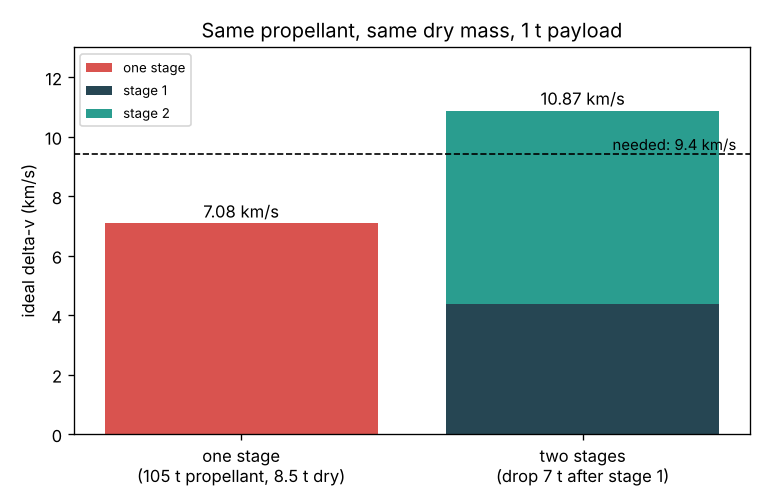
\includegraphics[width=0.85\linewidth]{figures/s01_staging.png}\\\small Same propellant and dry mass: two stages give 10.87 km/s, one stage only 7.08 km/s.\end{center}

\subsection*{E. Worked example}
(a) An engine has Isp = 300 s. Find ve, and the delta-v of a single stage that goes from 100 t to 25 t. (b) Find the speed of a circular orbit at 200 km. (c) Find the delta-v of the teaching launcher's stage 2 (15 t propellant, 1.5 t dry, Isp 340 s, 1 t payload).
\begin{enumerate}[nosep]
\item ve = 300 x 9.80665 = 2942 m/s.
\item Mass ratio = 100 / 25 = 4, and ln 4 = 1.386, so delta-v = 2942 x 1.386 = 4078 m/s. (Check: 4 = 2 x 2, so delta-v = 2 ve ln 2 = 2 x 2942 x 0.693 = 4078 m/s.)
\item r = 6371 + 200 = 6571 km = 6.571 x 10\textasciicircum{}6 m; v = sqrt(3.986 x 10\textasciicircum{}14 / 6.571 x 10\textasciicircum{}6) = sqrt(6.066 x 10\textasciicircum{}7) = 7788 m/s.
\item Stage 2 full: 1 + 15 + 1.5 = 17.5 t. Empty: 1 + 1.5 = 2.5 t. Mass ratio 7, ln 7 = 1.946.
\item ve = 340 x 9.80665 = 3334 m/s, so delta-v = 3334 x 1.946 = 6488 m/s.
\end{enumerate}
\textbf{Answer.} ve = 2942 m/s and delta-v = 4078 m/s; orbital speed at 200 km is 7788 m/s; stage 2 gives 6488 m/s.

\subsection*{F. Questions}
\begin{enumerate}[nosep]
\item \textbf{Conceptual.} Why does staging give more delta-v than one big stage with the same total propellant and the same total dry mass?
\item \textbf{Numerical.} An upper stage has Isp = 450 s. What mass ratio does it need to give 4000 m/s? If it carries 2 t of payload plus 1 t of dry mass, how much propellant must it hold?
\item \textbf{Graph and simulation interpretation.} On the rocket-equation figure, follow the Isp 300 s curve. How much delta-v do you gain going from a mass ratio of 2 to 4, and from 10 to 20? What does this tell you about adding more propellant?
\item \textbf{Design and optimisation challenge.} Design: you have 110 t of propellant to share between two stages (dry mass 8 percent of each stage's propellant, Isp 290 s and 340 s, payload 1 t). Try putting 80, 95 and 105 t in stage 1. Which split gives the most delta-v, and why is there a best split at all?
\end{enumerate}

\section{Session 2: Straight up: gravity and drag losses}

\subsection*{A. Real-world problem}
Session 1 said our two-stage teaching launcher has about 10.9 km/s of ideal delta-v, more than the 7.8 km/s of orbital speed. But a real rocket starts on a launch pad. Gravity pulls it down every second the engines burn, and the air pushes back while it is low and fast. How much speed do these two really take, why must a rocket's thrust be larger than its weight, and what happens if the rocket simply flies straight up? (A simplified teaching model, not a flight-planning method.)

\subsection*{B. Concept and theory}
On the pad the engine must first hold the rocket up: the thrust-to-weight ratio TWR = F / (m g0) must be above 1, and the net upward acceleration is (TWR - 1) g0. The engine burns propellant at the rate mdot = F / ve, so a stage with propellant m\_p burns for t\_b = m\_p / mdot. Flying straight up with constant gravity and no air, Newton's second law m dv/dt = F - m g integrates to v(t) = ve ln(m0 / m) - g t: the rocket equation minus g t. At burnout the missing speed g t\_b is the gravity loss; the longer the burn, the larger it is, so a higher TWR (a faster burn) loses less. After burnout the rocket coasts up a further v\_b\textasciicircum{}2 / (2 g). In general we cannot integrate by hand, so we step in time: with Euler's method each step uses the slope at its start (new v = v + a dt), which is simple but drifts; Runge-Kutta 4 (RK4) takes four slopes across the step and averages them, and is far more accurate for the same dt. Then we can add what the formula left out: gravity that weakens as G M / (R + h)\textasciicircum{}2, and drag D = 0.5 rho v\textasciicircum{}2 Cd A with air density rho = rho0 exp(-h / H) falling with height (scale height H = 8.5 km). Drag matters only low down; above about 50 km the air is too thin. Whatever we do, a rocket that only goes up has no sideways speed and must fall back.

\begin{itemize}[nosep]
\item TWR: thrust-to-weight ratio F / (m g0) (no unit)
\item mdot: propellant mass flow F / ve (kg/s)
\item t\_b: burn time m\_p / mdot (s)
\item g: gravity, g0 or G M / (R + h)\textasciicircum{}2 (m/s2)
\item D, Cd A: drag force and drag area (N, m2)
\item rho, H: air density and scale height (8500 m) (kg/m3, m)
\item dt: time step of the numerical method (s)
\end{itemize}

\begin{equation*}
\mathrm{TWR} = \frac{F}{m g_0},\qquad \dot m = \frac{F}{v_e},\qquad t_b = \frac{m_p}{\dot m}
\end{equation*}

\begin{equation*}
v(t) = v_e \ln\frac{m_0}{m(t)} - g\,t
\end{equation*}

\begin{equation*}
h(t) = v_e t - v_e\frac{m(t)}{\dot m}\ln\frac{m_0}{m(t)} - \tfrac12 g t^2
\end{equation*}

\begin{equation*}
m\frac{dv}{dt} = F - m\,g(h) - \tfrac12\rho_0 e^{-h/H} v|v|\,C_d A
\end{equation*}

\begin{equation*}
\text{gravity loss} = \int_0^{t_b} g\,dt \;=\; g\,t_b\ \text{(constant } g)
\end{equation*}

\begin{center}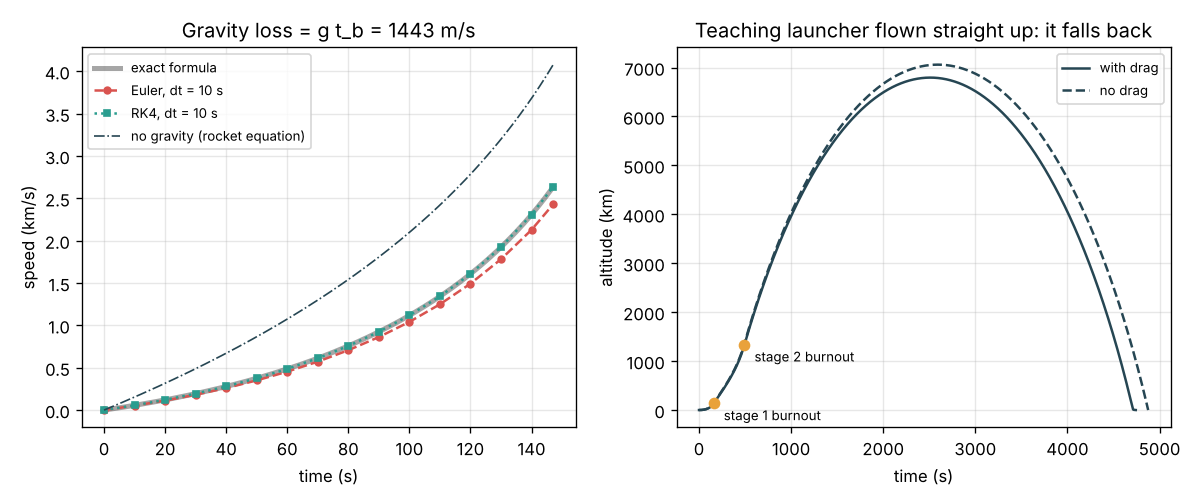
\includegraphics[width=0.85\linewidth]{figures/s02_vertical_flight.png}\\\small Left: exact, Euler and RK4 speeds; the gap to the rocket equation is the gravity loss. Right: the launcher flown straight up falls back.\end{center}

\subsection*{E. Worked example}
A single-stage rocket has m0 = 100 t, 75 t of propellant, Isp = 300 s and thrust F = 1.5 MN. It flies straight up with constant g0 and no air. Find the TWR, the burn time, the burnout speed and height, the gravity loss and the highest point.
\begin{enumerate}[nosep]
\item TWR = 1.5 x 10\textasciicircum{}6 / (100 000 x 9.80665) = 1.53. Above 1, so it lifts off.
\item ve = 300 x 9.80665 = 2942 m/s; mdot = 1.5 x 10\textasciicircum{}6 / 2942 = 509.9 kg/s; t\_b = 75 000 / 509.9 = 147.1 s.
\item Burnout speed: v = 2942 ln(100 / 25) - 9.80665 x 147.1 = 4078 - 1443 = 2636 m/s. The gravity loss is 1443 m/s.
\item Burnout height: h = 2942 x 147.1 - 2942 x (25 000 / 509.9) x 1.386 - 0.5 x 9.80665 x 147.1\textasciicircum{}2 = 432 755 - 199 980 - 106 094 = 126.7 km.
\item Coast: extra height = 2636\textasciicircum{}2 / (2 x 9.80665) = 354.2 km, so the top is 126.7 + 354.2 = 481 km. The numerical RK4 flight with dt = 1 s gives the same speed to 0.01 m/s.
\end{enumerate}
\textbf{Answer.} TWR 1.53, t\_b = 147.1 s, v\_b = 2636 m/s at 126.7 km, gravity loss 1443 m/s (35 percent of the ideal 4078 m/s), top of the flight 481 km.

\subsection*{F. Questions}
\begin{enumerate}[nosep]
\item \textbf{Conceptual.} Why does a rocket with a thrust-to-weight ratio of 1.1 waste so much propellant, even though it does lift off?
\item \textbf{Numerical.} The same 100 t rocket (75 t propellant, Isp 300 s) now has a 2.0 MN engine. Find the TWR, the burn time, the gravity loss and the burnout speed (constant g, no air).
\item \textbf{Graph and simulation interpretation.} In the left panel, Euler with 10 s steps ends below the exact curve, and the gap grows with time. Why is Euler always low here, and what happens to its error if you halve dt?
\item \textbf{Design and optimisation challenge.} Design: choose the smallest thrust for the 100 t stage (75 t propellant, Isp 300 s) that keeps the gravity loss below 1000 m/s. Lift-off TWR must also stay at or below 2.5 (load limit). Is there a design that meets both? Then switch on drag in the app: what new cost appears as TWR rises?
\end{enumerate}

\section{Session 3: Fly to orbit with a gravity turn and staging}

\subsection*{A. Real-world problem}
Session 2 showed that a rocket flown straight up falls back, however high it goes. To stay up it must end above the air moving sideways at about 7.8 km/s. So the rocket must turn over on the way up. Turn too early and it ploughs through thick air and falls into the sea; turn too late and gravity eats its propellant while it climbs. Can we fly our two-stage teaching launcher to a 200 km orbit, check the simulation against the laws it must obey, and find the largest payload it can carry? (A simplified teaching model, not a mission design tool.)

\subsection*{B. Concept and theory}
Put the Earth's centre at the origin and the launch site at the top of the circle. The rocket is a point with position r = (x, y), velocity v and mass m, and three forces act: thrust F along a pointing direction d chosen by the guidance, gravity -G M m r / |r|\textasciicircum{}3 that weakens with height, and drag D = 0.5 rho v\textasciicircum{}2 Cd A against the velocity. Mass falls at F / (Isp g0). The guidance has four phases. A short vertical rise clears the pad. A pitch kick tilts the thrust a few degrees east for 10 s. Then the gravity turn: the thrust points along the velocity, and gravity bends the path over by itself, so there is no sideways push in the thick air. After stage 1 burns out it is dropped, and stage 2 flies mostly sideways, pitching up just enough to hold the altitude near 200 km while it builds speed. Its engine cuts off when the orbital energy v\textasciicircum{}2 / 2 - G M / r equals that of a 200 km circular orbit. The orbit follows from two conserved quantities: energy fixes the semi-major axis a = -G M / (2 eps), and angular momentum h = |r x v| fixes the eccentricity, so perigee = a (1 - e) and apogee = a (1 + e). To validate, we integrate four rates alongside the motion: the ideal term F / m, the gravity loss g sin(gamma), the drag loss D / m and the steering loss (F / m)(1 - cos(alpha)), where gamma is the flight-path angle and alpha the angle between thrust and velocity. Their combination must equal the final speed, the ideal term must match the Session 1 rocket equation, and a coast after cut-off must keep its energy constant.

\begin{itemize}[nosep]
\item d: unit vector of the thrust direction (no unit)
\item kick: pitch-kick angle from vertical (degrees)
\item gamma: flight-path angle above the local horizontal (degrees)
\item alpha: angle between thrust and velocity (degrees)
\item eps: specific orbital energy v\textasciicircum{}2 / 2 - mu / r (J/kg)
\item a, e: semi-major axis and eccentricity of the orbit (m, no unit)
\item q: dynamic pressure 0.5 rho v\textasciicircum{}2 (Pa)
\end{itemize}

\begin{equation*}
m\,\ddot{\mathbf r} = F\,\mathbf d - \frac{\mu m}{|\mathbf r|^3}\,\mathbf r - \tfrac12\rho(h)\,|\mathbf v|\,\mathbf v\,C_d A,\qquad \dot m = -\frac{F}{I_{sp} g_0}
\end{equation*}

\begin{equation*}
\mathbf d = \frac{\mathbf v}{|\mathbf v|}\quad\text{(gravity turn)}
\end{equation*}

\begin{equation*}
\varepsilon = \frac{v^2}{2} - \frac{\mu}{r},\qquad a = -\frac{\mu}{2\varepsilon},\qquad e = \sqrt{1 + \frac{2\varepsilon h^2}{\mu^2}}
\end{equation*}

\begin{equation*}
h_p = a(1-e) - R_E,\qquad h_a = a(1+e) - R_E
\end{equation*}

\begin{equation*}
v_{\mathrm{final}} = \int \frac{F}{m}dt - \int g\sin\gamma\,dt - \int \frac{D}{m}dt - \int \frac{F}{m}(1-\cos\alpha)\,dt
\end{equation*}

\begin{center}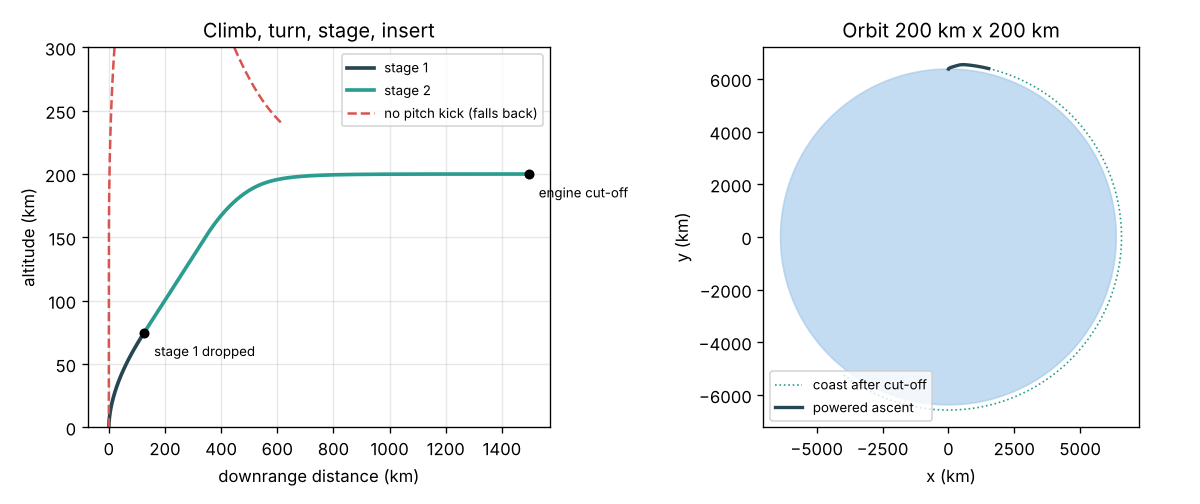
\includegraphics[width=0.85\linewidth]{figures/s03_ascent.png}\\\small Left: the climb, turn, staging and cut-off. Right: the coast after cut-off is a 200 km orbit.\end{center}

\subsection*{E. Worked example}
Fly the reference launch: kick 3 degrees, payload 1 t, target 200 km. Hand-check the staging time and the orbital speed, then check the simulation's delta-v budget.
\begin{enumerate}[nosep]
\item Stage 1 burn time: mdot = 1.6 x 10\textasciicircum{}6 / (290 x 9.80665) = 562.6 kg/s, so t\_b = 90 000 / 562.6 = 160.0 s. The simulation stages at t = 160.0 s, at 74.8 km and 3195 m/s.
\item Circular speed at 200 km (Session 1): sqrt(3.986 x 10\textasciicircum{}14 / 6.571 x 10\textasciicircum{}6) = 7788 m/s. The simulation cuts off at 7788 m/s, at 200.0 km, after 472 s.
\item The orbit: perigee 199.8 km, apogee 200.2 km, eccentricity below 0.0001. A 3000 s coast keeps its energy to 1 part in 10\textasciicircum{}14.
\item Budget: ideal 9801 - gravity 1442 - drag 95 - steering 476 = 7788 m/s, equal to the final speed to within 0.1 m/s.
\item Rocket equation for the propellant used (stage 1 all 90 t, stage 2 14.05 t, 949 kg left): 290 g0 ln(114.5 / 24.5) + 340 g0 ln(17.5 / 3.449) = 4385 + 5415 = 9801 m/s, the same as the ideal term.
\end{enumerate}
\textbf{Answer.} Orbit 199.8 x 200.2 km at 7788 m/s; losses 2013 m/s in total (gravity 72 percent of them); 949 kg of stage-2 propellant left as margin.

\subsection*{F. Questions}
\begin{enumerate}[nosep]
\item \textbf{Conceptual.} Why does a gravity turn (thrust along the velocity) waste less propellant than pointing the rocket at a fixed angle from the start?
\item \textbf{Numerical.} A satellite is in a circular orbit at 400 km instead of 200 km. Find its speed. Then, ignoring losses, how much less sideways speed does it need than at 200 km, and why does it still need more energy to get there?
\item \textbf{Graph and simulation interpretation.} In the pitch-kick window, both 1.5 degrees and 4.5 degrees fail. Using the trajectory and budget views of the app, explain the two different ways they fail.
\item \textbf{Design and optimisation challenge.} Design: the customer's satellite is 2000 kg. Using the model, choose the pitch kick, and say how much propellant margin is left. Then propose one change to stage 2 (more propellant, or higher Isp) that gives at least 500 kg of propellant margin, and check it in the app or with `launch`.
\end{enumerate}

\section{Real-world mini-project}
\textbf{How much payload can the teaching launcher put in orbit?} A small-satellite customer asks how heavy a satellite the teaching launcher can carry to a 200 km orbit. Use `launch` and `max\_payload` from Session 3 with the standard stages, a pitch kick chosen from 2, 2.5 and 3 degrees, and payloads in steps of 250 kg. Count a flight as successful only if its perigee is above 150 km. Then the customer asks what a hydrogen upper stage (Isp 450 s, same masses) would change. These are illustrative numbers, not a real vehicle's performance.

\section{The path ahead}
\begin{enumerate}[nosep]
\item \textbf{Session 4: Launch from a rotating Earth.} Give the rocket the surface speed of its launch latitude and compute drag with the air speed (velocity minus the rotating air).
\item \textbf{Session 5: Thrust that changes with altitude.} Stages described by vacuum thrust, vacuum Isp and exit area, with the outside pressure from the exponential atmosphere.
\item \textbf{Session 6: Max Q and throttling.} A throttle law for stage 1 that keeps q below a chosen limit, with the burn lengthened to use all the propellant.
\item \textbf{Session 7: An optimised upper-stage steering law.} Replace the altitude hold with tan(pitch) = a - b t and search a and b (and the kick) to maximise payload to a 200 km circular orbit.
\item \textbf{Session 8: The animated Target flight.} A Matplotlib or browser animation: the rocket over a curved Earth, the first stage falling away after separation, and live altitude, speed, dynamic pressure and delta-v budget panels.
\end{enumerate}

\section{Answers and hints}

\subsection*{Session 1}
\begin{enumerate}[nosep]
\item \textbf{Conceptual.} Hint: What does the rocket still carry, late in the flight, if it never drops anything? Solution: The rocket equation depends on the mass ratio m0 / mf. A single stage must carry all of its empty tanks and engines to the very end, so mf is large and the ratio is poor. A staged rocket drops stage 1's dry mass when it is empty; stage 2 then starts light and ends very light, so its own mass ratio is large. The ideal delta-v values of the stages add. With the teaching launcher: 10 873 m/s staged against 7079 m/s unstaged.
\item \textbf{Numerical.} Hint: Turn the rocket equation round: m0 / mf = exp(delta-v / ve). Solution: ve = 450 x 9.80665 = 4413 m/s. m0 / mf = exp(4000 / 4413) = exp(0.906) = 2.475. The empty mass mf = 2 + 1 = 3 t, so m0 = 3 x 2.475 = 7.43 t and the propellant is 7.43 - 3 = 4.43 t. Check: 4413 x ln(7.43 / 3) = 4413 x 0.907 = 4000 m/s.
\item \textbf{Graph and simulation interpretation.} Hint: Doubling the mass ratio always adds ve ln 2. Solution: Both steps double the mass ratio, so each adds ve ln 2 = 2942 x 0.693 = 2039 m/s. But going from 2 to 4 means adding propellant equal to twice the empty mass, while going from 10 to 20 means adding ten times the empty mass. The same extra speed costs five times more propellant at high mass ratios: the curve flattens. Diminishing returns are why one stage cannot reach orbit.
\item \textbf{Design and optimisation challenge.} Hint: Use `stack\_delta\_v` from the lesson in a loop over the stage-1 propellant, or the Session 1 app with matching dry masses. Solution: With 8 percent dry mass: 80 t in stage 1 gives 3134 + 7618 = 10 752 m/s; 95 t gives 4479 + 6857 = 11 336 m/s; 105 t gives 5947 + 5067 = 11 015 m/s. A loop in steps of 5 t finds the best near 100 t (5119 + 6269 = 11 389 m/s). Too small a stage 1 has a poor mass ratio because it must lift a heavy stage 2; too small a stage 2 has a poor mass ratio because its own dry mass and the payload dominate. The best split balances the two. Trade-off: the ideal delta-v is not the whole story, because a big stage 1 needs a lot of thrust and the losses of Session 2 depend on how long each stage burns.
\end{enumerate}

\subsection*{Session 2}
\begin{enumerate}[nosep]
\item \textbf{Conceptual.} Hint: What is the net upward acceleration at TWR 1.1, and what does gravity do during every second of the burn? Solution: At TWR 1.1 only one tenth of the thrust accelerates the rocket; the rest just holds it up against gravity. The burn takes a long time and gravity removes g0 = 9.8 m/s of speed every second. For the worked-example stage the gravity loss is 1839 m/s at TWR 1.2 against 919 m/s at TWR 2.4. A higher TWR burns faster and loses less, but needs bigger, heavier engines and gives higher loads in the thick air: real rockets lift off at about 1.2 to 1.6 and accelerate harder later.
\item \textbf{Numerical.} Hint: mdot = F / ve; t\_b = m\_p / mdot; v\_b = ve ln 4 - g0 t\_b. Solution: TWR = 2.0 x 10\textasciicircum{}6 / 980 665 = 2.04. mdot = 2.0 x 10\textasciicircum{}6 / 2942 = 679.8 kg/s; t\_b = 75 000 / 679.8 = 110.3 s. Gravity loss = 9.80665 x 110.3 = 1082 m/s. v\_b = 4078 - 1082 = 2997 m/s. Check: 33 percent more thrust cut the loss by 361 m/s (from 1443 m/s) and the speed rose by the same amount.
\item \textbf{Graph and simulation interpretation.} Hint: Is the acceleration rising or falling during the burn? Euler uses the value at the start of each step. Solution: The rocket gets lighter, so its acceleration F / m - g keeps rising. Euler uses the acceleration at the start of each step, which is always the smallest in that step, so every step adds too little speed and the errors pile up. Euler is a first-order method: halving dt halves the error (22.5 m/s at dt = 1 s, 11.4 m/s at 0.5 s; the checkpoint tests this). RK4 is fourth order: halving dt divides its error by about 16, so even 10 s steps look exact on the graph.
\item \textbf{Design and optimisation challenge.} Hint: Gravity loss = g0 m\_p ve / F, so F = g0 m\_p ve / loss. Solution: F = 9.80665 x 75 000 x 2942 / 1000 = 2.164 MN, so TWR = 2.21. Both limits are met for thrusts from 2.164 to 2.45 MN (TWR 2.21 to 2.5); the smallest is 2.164 MN, about 2.17 MN after rounding up. With drag on, a faster rocket reaches high speed while still in thick air, so the drag loss and the dynamic pressure grow with TWR. The design is a trade between gravity loss (wants high TWR) and drag and structural load (want low TWR), plus the mass of bigger engines, which this model does not include.
\end{enumerate}

\subsection*{Session 3}
\begin{enumerate}[nosep]
\item \textbf{Conceptual.} Hint: Look at the steering-loss term (F / m)(1 - cos alpha), and think about the sideways force on the rocket in thick air. Solution: In a gravity turn the thrust is along the velocity, so alpha = 0 and the steering loss is zero: every newton of thrust adds speed. Gravity does the turning for free by bending the path. A fixed-angle climb pushes partly across the velocity, which changes direction instead of speed, and in thick air the angle between body and airflow causes large sideways loads that can break the rocket. In the reference flight the steering loss (476 m/s) comes almost entirely from the stage-2 altitude hold and the short pitch kick, not from stage 1.
\item \textbf{Numerical.} Hint: v = sqrt(mu / r); compare the energy eps = -mu / (2 r) for the two orbits. Solution: r = 6771 km, so v = sqrt(3.986 x 10\textasciicircum{}14 / 6.771 x 10\textasciicircum{}6) = sqrt(5.887 x 10\textasciicircum{}7) = 7673 m/s, which is 115 m/s less than 7788 m/s. But the energy per kg is eps = -mu / (2 r): -30.33 MJ/kg at 200 km and -29.43 MJ/kg at 400 km, so the higher orbit needs 0.90 MJ/kg more. The rocket must climb higher (potential energy) even though it ends slower. Higher orbits always need more delta-v from the ground.
\item \textbf{Graph and simulation interpretation.} Hint: Compare the gravity and drag losses of the presets "No pitch kick" and "Too much kick" with the reference flight. Solution: With too little kick, stage 1 climbs nearly vertically, so it wastes speed against gravity (gravity loss rises) and stage 2 starts high and steep but slow sideways; it runs out of propellant before reaching 7.8 km/s. With too much kick the rocket turns over while still low, flies fast through thick air (drag loss of thousands of m/s and a dynamic pressure above 300 kPa, which a real rocket would not survive) and falls back before it can climb. The window between them, 2 to 4 degrees in this model, is narrow, which is why real pitch programs are planned carefully.
\item \textbf{Design and optimisation challenge.} Hint: Run `launch(payload=2000, kick=k)` for k = 2, 2.5 and 3 and read `prop\_left`; then pass a modified `stages` list. Solution: Only the 2.5 degree kick reaches orbit with 2000 kg, with a perigee of 162 km and 0 kg of propellant left: no margin at all, which no real mission would accept. With an Isp 450 s upper stage the same flight reaches orbit with about 1650 kg left. Trade-offs: more stage-2 propellant makes stage 1 heavier and lowers its TWR, and a hydrogen stage has bulky tanks (more dry mass) than this model assumes. A margin is needed because the real atmosphere, thrust and steering will differ from the model.
\end{enumerate}

\section{How to join}
Read \texttt{CONTRIBUTING.md} in the repository, then pick an issue labelled \texttt{good first issue}. Repository: \url{https://github.com/KrunalPanchal1995/pan-iit-oss/tree/main/openascent}

\end{document}
